Uno dei protocolli del livello applicativo più utilizzati in Internet è \verb+HTTP+ (\textit{HyperText Transfer Protocol}).
Si basa sul pattern sincrono richiesta/risposta (\textit{client}/\textit{server}): il \textit{client} effettua una richiesta e il \textit{server} restituisce una risposta.
Vi sono quindi due tipi di messaggi: messaggi di richiesta e messaggi di risposta.

Grazie agli strati sottostanti, \verb+HTTP+ non deve occuparsi di come avvengono le connessioni, ma definire una ben definita sintassi fra i vari utilizzatori.
A sua volta, questo protocollo viene utilizzato come base su cui disporre ulteriori strutture e/o architetture, dove \verb+SOAP+, \verb+RCP+ e \verb+RESTful+ sono alcuni esempi.

Il paradigma richiesta/risposta permette un'unica direzionalità nel flusso dati, definito nello standard \verb+HTTP/1.0+, nel quale alla ricezione della risposta, la connessione viene conclusa \cite{Rfc1945}.
Se si volesse interrogare successivamente il servizio, sarebbe necessario creare una nuova connessione.
Solo nella versione aggiornata dello standard \verb+HTTP/1.1+, viene data la possibilità di non chiudere immediatamente il collegamento \cite{Rfc2068}.
Queste connessioni persistenti \textit{KeepAlive} possono essere lasciate aperte un numero prefissato di secondi ed utilizzate in seguito per altre richieste.
Mantenendo aperta la comunicazione, è possibile inviare richieste multiple senza aspettare la risposta di ognuna, con un meccanismo di pipeline; il \textit{server} dovrà inviare le risposte nello stesso ordine di ricezione \cite{Rfc7230}.

Nella nuova versione dello standard \verb+HTTP/2+, è permessa la comunicazione preventiva tramite meccanismo di \verb+Server Push+ \cite{Rfc7540}.
Viene data la possibilità di soddisfare più richieste contemporanee che sono necessarie per concludere la richiesta originale.
Questo è possibile solamente quando il \textit{server} riesce a stabilire a priori le successive richieste, come possono essere le immagini allegate ad una pagina web.

\begin{figure}[H]
  \centering
  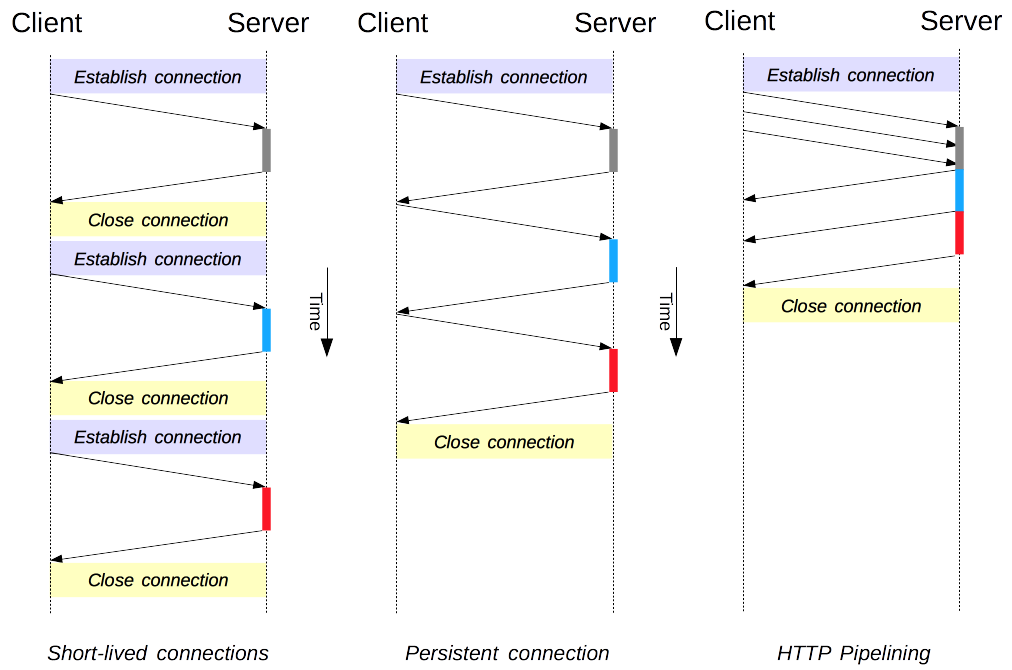
\includegraphics[width=0.95\linewidth, keepaspectratio]{http}
  \caption{Modello delle diverse tipologie di connessioni sincrone HTTP}
  \label{fig:http}
\end{figure}

\subsection{WebSocket}
\label{subsec:httpWebsocket}

Nonostante la possibilità di tenere aperta la connessione tra i due interlocutori, il paradigma sincrono richiesta/risposta rimane invariato e non è mai il \textit{server} che invia informazioni al \textit{client} senza un'esplicita richiesta iniziale.
Il \textit{client}, quindi, può accorgersi di un certo cambiamento solamente inviando richieste multiple \verb+XMLHttpRequest+ o \verb+<iframe>s+ in un determinato lasso di tempo con lunghi periodi di polling e aprendo più connessioni \cite{Rfc6202}.

Per venire incontro a questa esigenza è stato introdotto il \verb+WebSocket+, una tecnologia che fornisce una comunicazione bidirezionale \textit{full-duplex} tra i due interlocutori utilizzando una singola connessione \verb+TCP+ \cite{Rfc6455}.
Infatti il \verb+WebSocket+ è un protocollo indipendente, la cui unica correlazione con l'\verb+HTTP+ è nel modo in cui fa l'\textit{handshake} durante una richiesta \textit{Upgrade} verso il \textit{server}.
La comunicazione viene mantenuta aperta da entrambe le parti e chiusa solo tramite richieste esplicita o problemi di rete.
Lo scambio di informazioni si trasforma da sincrono ad asincrono, dove gli interlocutori possono inviare richieste anche se non interrogati.

Di particolare nota sono i \verb+SSE+ (\textit{Server-sent events}).
Una tecnologia non ancora supportata da tutti i browser, che permette l'invio di notifiche \verb+Push+ asincrone da parte del \textit{server} a seguito di una richiesta esplicita iniziale \cite{SSE}.
Il \textit{client} non chiude immediatamente la comunicazione e rimane in attesa senza intervenire delle successive notifiche.

\begin{figure}[H]
  \centering
  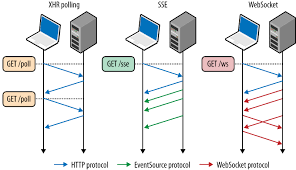
\includegraphics[width=0.95\linewidth, keepaspectratio]{websocket}
  \caption{Diversi approcci del pattern di comunicazione sincrona rispetto asincrona}
  \label{fig:websocket}
\end{figure}
